\documentclass[letterpaper,conference, 10pt]{ieeeconf}
\usepackage[T1]{fontenc}
\usepackage[latin9]{inputenc}
\usepackage{calc}
\usepackage{amssymb}
\usepackage{graphicx}
\usepackage{xcolor}
\usepackage{mathtools}
% \usepackage[caption=false,font=footnotesize]{subfig}
\usepackage{cite}
\usepackage[unicode=true,
 bookmarks=true,bookmarksnumbered=true,bookmarksopen=true,bookmarksopenlevel=1,
 breaklinks=false,pdfborder={0 0 0},pdfborderstyle={},backref=false,colorlinks=false]
 {hyperref}
% \hypersetup{pdftitle={Your Title},
%  pdfauthor={Your Name},
%  pdfpagelayout=OneColumn, pdfnewwindow=true, pdfstartview=XYZ, plainpages=false}
 \usepackage[capitalise]{cleveref}
 \usepackage{amsmath}
 \usepackage{subcaption}
 \interdisplaylinepenalty=2500

\makeatletter
\makeatother

\DeclareMathOperator*{\argmin}{arg\,min}

\begin{document}

\title{Optimal Trajectory Generation for Exploration of Three Dimensional Spaces}

\author{Brendon Forsgren$^1$, Seth Nielsen$^2$, Thane Downing$^2$}
\thanks{$^1$ Brendon Forsgren is with the Department of Mechanical Engineering, Brigham Young University}%}
\thanks{$^{2} $Seth Nielsen and Thane Downing are with the Department of Electrical and Computer Engineering, Brigham Young University}%

\maketitle

\begin{abstract}
Trajectory generation and path planning are an important part of UAV autonomy, and the ability to successfully determine the path to complete a mission is an open research area. Many techniques require previous knowledge of the environment to ensure a collision free path while others seek to be able to generate trajectories and re-plan in real-time to avoid obstacles. We present a framework that allows a quadrotor UAV to explore a sparsely populated, unknown region given a set of target waypoints. Our framework determines the best order to visit the target points to minimize the distance traveled and generates dynamically feasible trajectories while avoiding obstacles without assuming any prior knowledge of the environment. We demonstrate the results of our framework with a simulation that generates a random map with a predetermined number of waypoints to hit and show the generated trajectories.
\end{abstract}

\section{Introduction}

The ability of a UAV to navigate autonomously in an unmapped region has many different subproblems including trajectory generation, waypoint selection, control and state estimation. Different conditions, such as the absence of GNSS make this problem difficult as generating an accurate map and following a trajectory require accurate knowledge of the state of the UAV.

We motivate with an example of a damaged city after a natural disaster or a cavernous structure where the area can be assumed to be mostly empty but where either a map does not exist or a map may no longer be reliable. Exploration of the area may be required to assess damage, find people or another mission but the environment is potentially dangerous and as a result using a UAV to explore is desirable to not put human life at risk. In this work we tackle the problem of trajectory generation and selecting a desired order to visit our target destinations (i.e. the traveling salesman problem).

We assume that a bound on the area to be explored is known, that the target points have been previously selected and that we have perfect control of the UAV (i.e. our control inputs result in the expected change in state). Additionally, the UAV is equipped with some sensor that is able to detect and estimate the radius of an obstacle. \Cref{section:prev_work} does a brief literature review of trajectory generation and solving the traveling salesman problem, \cref{section:methods} describes the methods used in our framework. We then discuss results in \cref{section:results} and close with a discussion of improvements and future work.

\section{Previous Work}
\label{section:prev_work}

The traveling salesman problem (TSP) is an integer linear programming (ILP) problem that is classified as NP-hard, meaning that a brute force solution to the problem could require computational time that grows exponentially with the number of variables. The TSP is one of the most popular problems in the ILP community because despite the simplicity of the problem, it is quite difficult to generate a solution in a reasonable amount of time, especially as the number of cities to visit increases. Goyal \cite{goyal2010survey} and Laporte \cite{laporte1992traveling} perform surveys on the traveling salesman problem. They look at exact solutions, such as branch and bound algorithms, but note that the time complexity grows exponentially with the number of variables and are not suitable for anything except small versions of the problems. They also examine approximate methods that use heuristics to obtain a solution. These solutions are not guaranteed to be the optimal solution but have the advantage that they grow much slower with the number of design variables than exact approaches.

Recently there has been a large increase in the number of gradient free algorithms that can provide an approximate solution to the TSP. Mukhairez et al. in their work \cite{mukhairez2015performance} perform a comparison of three prominent algorithms including Simulated Annealing, a genetic algorithm, and Ant Colony optimization. The criteria they evaluated were execution time and the shortest distance found. Their results found that Simulated Annealing produced the fastest run time and returned the second shortest distance found on average. Ant Colony Optimization found the shortest distance but took the longest to run. Based on their results, we decided to use a Simulated Annealing algorithm to obtain an approximate solution to the TSP for our application.

Path planning and trajectory generation are well-researched topics in which many algorithms for generating trajectories exist. Several path planning algorithms, such as RRT, RRT$^*$, A$^*$, and Voronoi graph methods are used to generate straight line paths between a desired start and end point \cite{goerzen2010survey}. Many of the algorithms in \cite{goerzen2010survey} suffer from the limitation that they require a previous knowledge of the environment and are computationally complex enough that they cannot be run in real time. Additionally, in their generic form, many of these algorithms do not consider the dynamics of the UAV system being flown and as a result may generate dynamically infeasible trajectories unless the straight line path is sufficiently altered. This requires additional constraints on the planning process and can increase the time to generate a path.

Other approaches seek to generate an optimal trajectory with respect to some cost function that do take into account dynamic constraints. In \cite{chen2016uav} an artificial potential field method is reconstructed into an unconstrained problem allowing for the solution to be found efficiently. \cite{roberge2012comparison} compares gradient free algorithms for real time path planning of UAV's that take the dynamics of the vehicle into consideration. Our approach follows the work done by \cite{mellinger2011minimum} which reduces the planning space using the differential flatness, a property which quadrotor UAV's have.

\section{Methodology}
\label{section:methods}

\subsection{Map Generation}
In order to build a realistic environment for the UAV to explore we generate a map ba

\subsection{Simulated Annealing}
As mentioned in the introduction, the order in which the given waypoints would be visited was determined via a simulated annealing optimization algorithm, which is explained below. Because of battery capacity, size, and weight constraints, the amount of flight time possible for one continuous flight of a multirotor is very limited; typically, on the order of 30 minutes or less. A full recharge or battery replacement has a high time cost, thus it is desirable that the route to visit all waypoints be as energy-efficient as possible. To simplify the problem, it was decided that solving for the shortest path through all waypoints would approximately have the outcome of minimal energy expenditure as well. The presence of obstacles were not considered for this portion of the problem.

The algorithm of simulated annealing gets its name from its analogous properties to the metallurgic process of annealing whereby metals must be cooled at a regular schedule in order to settle into their lowest energy state. The algorithm can be divided into the following steps:

\begin{enumerate}
  \item Randomly select waypoints from the given set and swap their placement in the sequence
  \item Compute the total distance of the route; begin at the first waypoint in the sequence, calculate the Euclidean distance from each waypoint to the next --- including from the final waypoint back to the starting point --- then take the sum of all the distances
  \item Compare the route length to the previous route's and decide whether to accept the new route or reject it based on the current temperature and the amount of improvement. To be accepted, one of the following requirements must be met:
    \begin{itemize}
        \item The route must be an improvement over the current route (i.e. must be shorter)
        \item The route is somewhat longer, but is within the bounds determined by the current temperature and how much longer the new route is
    \end{itemize}
  \item Repeat until the max number of steps $n$ has been reached 
\end{enumerate}

The algorithm was initialized by sorting the generated waypoints in random order and prepending the origin $(0,0,0)$ as the starting point. 

There were three tunable parameters for the algorithm: the initial temperature $T_{\text{max}}$, the final temperature $T_\text{min}$, and the number of iterations to run $n$. These were automatically tuned by exploring the search space prior to initializing the algorithm and determining a reasonable $T_{\text{max}}$ and $T_\text{min}$ as well as assessing how long one iteration takes. The desired total length of time was set manually by the user. Throughout the algorithm, the temperature decreased exponentially according to the following equation:

\begin{equation}
\begin{aligned}
  T = T_{\text{max}}e^{T_{c}r} \\
  \label{eq:temp}
  \end{aligned}
\end{equation}

where 
\begin{equation}
\begin{aligned}
  T_{c} = -\ln{\frac{T_{\text{max}}}{T_{\text{min}}}} \\
  \label{eq:t_c}
  \end{aligned}
\end{equation}
and $r$ is the ratio of the current iteration to the set total number of iterations $n$. A new route was accepted probabalistically based on the truth value of the output of the following expression: 

\begin{equation}
\begin{aligned}
  \text{e}^{\frac{-\delta d}{T}} < x \\
  \label{eq:t_c}
  \end{aligned}
\end{equation}
where $x$ is a random value taken from a uniform distribution of values between $0$ and $1$.

\subsection{Trajectory Generation}

This section details how dynamically feasible trajectories are generated between successive waypoints. The next subsection, \cref{subsection:diff_flat} gives a brief overview of differential flatness, a property of some dynamical systems that more easily allows for feasible trajectory generation. Lastly we discuss the optimization problem in \cref{subsection:opt_prob} and how it is solved.

\subsubsection{Differential Flatness}
\label{subsection:diff_flat}

A nonlinear system is defined by \cref{eq:xdot}
\begin{equation}
\begin{aligned}
  \dot{x} = f(x,u),\\
  \label{eq:xdot}
  \end{aligned}
\end{equation}
where $x \epsilon \mathbb{R}^n$ is the system state, $u \epsilon \mathbb{R}^m$ the inputs and, $\dot{x}$ the time derivative of the state. The system is differentially flat if there are $m$ output functions (called flat outputs) such that all of the states and inputs can be expressed in terms of the $m$ flat outputs and their derivatives. This implies that if a desired trajectory can be defined for the $m$ flat outputs, then all the states and inputs for that trajectory can be calculated. This simplifies the planning space from $n$ dimensions to $m$ dimensions.

A quadrotor's state vector and input vector are defined as
\begin{align*}
    \boldsymbol{x}&=[x,y,z,\dot{x},\dot{y},\dot{z},\phi,\theta,\psi,\dot{\phi},\dot{\theta},\dot{\psi}]^T,\\
    \boldsymbol{u}&=[F, \tau_x, \tau_y, \tau_z]^T,
\end{align*}
where $x, y, z$ are the inertial positions, $\phi, \theta, \psi$ are the roll, pitch and yaw angles respectively. $F$ is the force along the body $z$ axis and $\tau_i$ is the torque along the body $i$ axis.

Using the flat outputs $\boldsymbol{x}_{out}=[x, y, z, \psi]^T$ it has been shown \cite{mellinger2011minimum} that the quadrotor system is differentially flat and that trajectory planning can be done in the four dimensional space of the flat outputs instead of the 12 dimensional space of the state.

\subsubsection{Optimization Problem}
\label{subsection:opt_prob}

The goal of the optimization is to find a minimum snap trajectory using the flat outputs. The choice to minimize snap as explained in \cite{mellinger2011minimum} is because the all derivatives up to the fourth derivative of the flat outputs are required to fully define the inputs and states of the quadrotor system. See \cite{mellinger2011minimum} for a more in depth derivation. Since four derivatives are required, we chose to define the trajectories of our flat outputs using quintic polynomials where each output has the following form 
\begin{equation*}
    B(t) = p_{B,0} + p_{B,1}t + p_{B,2}t^2 + p_{B,3}t^3 + p_{B,4}t^4 + p_{B,5}t^5
\end{equation*}
where $B$ can be replace with the corresponding flat output and $p_{B,i}$ are the coefficients of the polynomial. These coefficients become our design variables in the optimization. Our cost function appears in \cref{eq:min_snap_cost} and uses some time step $dt$ between evaluation points in the summation.

\begin{equation}
    J = \argmin_p \sum_{t_0}^{t_f} \ddddot{x}(t)^2 + \ddddot{y}(t)^2 + \ddddot{z}(t)^2 + \ddddot{\psi}(t)^2
    \label{eq:min_snap_cost}
\end{equation}

Constraints were placed on the position and velocity of the initial and final starting point. A heuristic was used to put the constraint on the final velocity that constrained the quadrotor be moving in the forward direction after the yaw rotation was applied. The velocity at the end of all trajectory segments was constrained to be constant in magnitude. The constraints take the form found in \cref{eq:constraints}.
\begin{equation}
\begin{aligned}
    \boldsymbol{x}_{out}(0) &= \boldsymbol{x}_0\\
    \boldsymbol{\dot{x}}_{out}(0) &= \boldsymbol{{\dot{x}}}_0\\
    \boldsymbol{x}_{out}(t_f) &= \boldsymbol{x}_{t_f}\\
    \boldsymbol{\dot{x}}_{out}(t_f) &= \boldsymbol{{\dot{x}}}_{t_f}
\end{aligned}
    \label{eq:constraints}
\end{equation}
The above cost function and constraints can be reformulated as a quadratic program with the form found in \cref{eq:quad_prog}. Note that any constraint (equality or inequality) can be added as long as it fits the linear form. Possible other constraints include a maximum velocity or acceleration constraint.
\begin{align}
\begin{aligned}
    &\argmin_p \sum_{t_0}^{t_f} p^T H p + f^T p\\
    \centering
    &s.t.\ \ \ \ \ \ \ \ \ \ \ \ \ \ \ Ap = b
\end{aligned}
    \label{eq:quad_prog}
\end{align}
The last step before solving the equation was to determine values for $t_0$ and $t_f$. The value for $t_0$ was assumed to be $0$ for each segment of the trajectory. This was done because for long trajectories or trajectories with many segments resulted in coefficients that were very small (the order of $1e-20$ and smaller) and eventually became unusable. The final time, $t_f$, was chosen to be equal to the distance between points under the assumption that the quadrotor would be traveling at an average speed of greater than $1\frac{m}{s}$ for the segment of the trajectory. The optimization problem described in \cref{eq:quad_prog} was solved using CVXPY \cite{cvxpy, cvxpy_rewriting}. %Unstable for really long flights

We note that the above formulation does not generate trajectories that avoid obstacles since a constraint to avoid a spherical obstacle is a non-linear constraint as in \cref{eq:obst_con} and cannot be handled by CVXPY which requires linear constraints.
\begin{equation}
    (x - x_{obst})^2 + (z - z_{obst})^2 + (z - z_{obst})^2 - r^2 \geq 0
    \label{eq:obst_con}
\end{equation}
To circumvent this we run the optimization using CVXPY and check the optimization against discovered obstacles. If there is a collision then the optimization is rerun using a non-convex solver using the pyOptSparse \cite{Perez2012a} with the SNOPT solver from Stanford. 

\section{Results}
\label{section:results}

% \subsection{Map Generation} %maybe we don't need a results of this??? 
% Yeah, it's pretty straightforward.  I'll put all the principles in the method section.  It can be assumed that when we hit run on a random number generator we will get the proper random numbers.

\subsection{Simulated Annealing}
The initial random path normally resulted in a total path length on the order of $~2,800 m$. 

\subsection{Trajectory Generation}

The trajectory generation was done in several experiments. The first shows the ability to successfully generate a trajectory between successive waypoints. The second demonstrates the ability to correctly switch optimizers to allow for obstacle avoidance. Lastly we demonstrate the ability to solve for trajectories on a large map with multiple obstacles.

The results of the first experiment can be seen in \cref{fig:optimal_traj}. As can be seen the generated trajectory does not require the UAV to stop and turn but instead defines a smooth path to transition the UAV from one waypoint to the next.
\begin{figure}[bth]
    \centering
    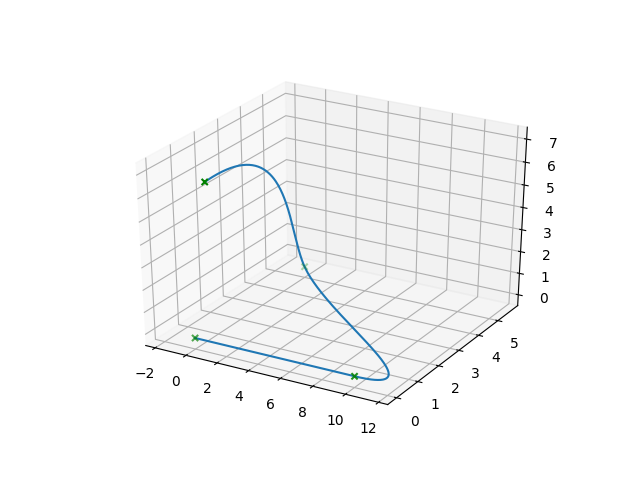
\includegraphics[scale=0.5]{traj.png}
    \caption{Minimum snap trajectory for 3 waypoints (2 segments). The waypoints are marked by a green x and the trajectory is in blue}
    \label{fig:optimal_traj}
\end{figure}

The next experiment demonstrated the ability to switch optimizers when obstacle avoidance was necessary and generate a new trajectory to avoid the obstacle. \Cref{fig:obst_avoid} shows the results. As can be seen in \cref{fig:diff_flat}, the original trajectory takes the UAV right through the zone designated to avoid. \Cref{fig:diff_flat_obst} begins by following the same trajectory but detects the obstacle when it becomes in range and successfully replans the trajectory to avoid it.

\begin{figure}[bth]
    \begin{subfigure}{0.5\textwidth}
          \centering
          % include first image
          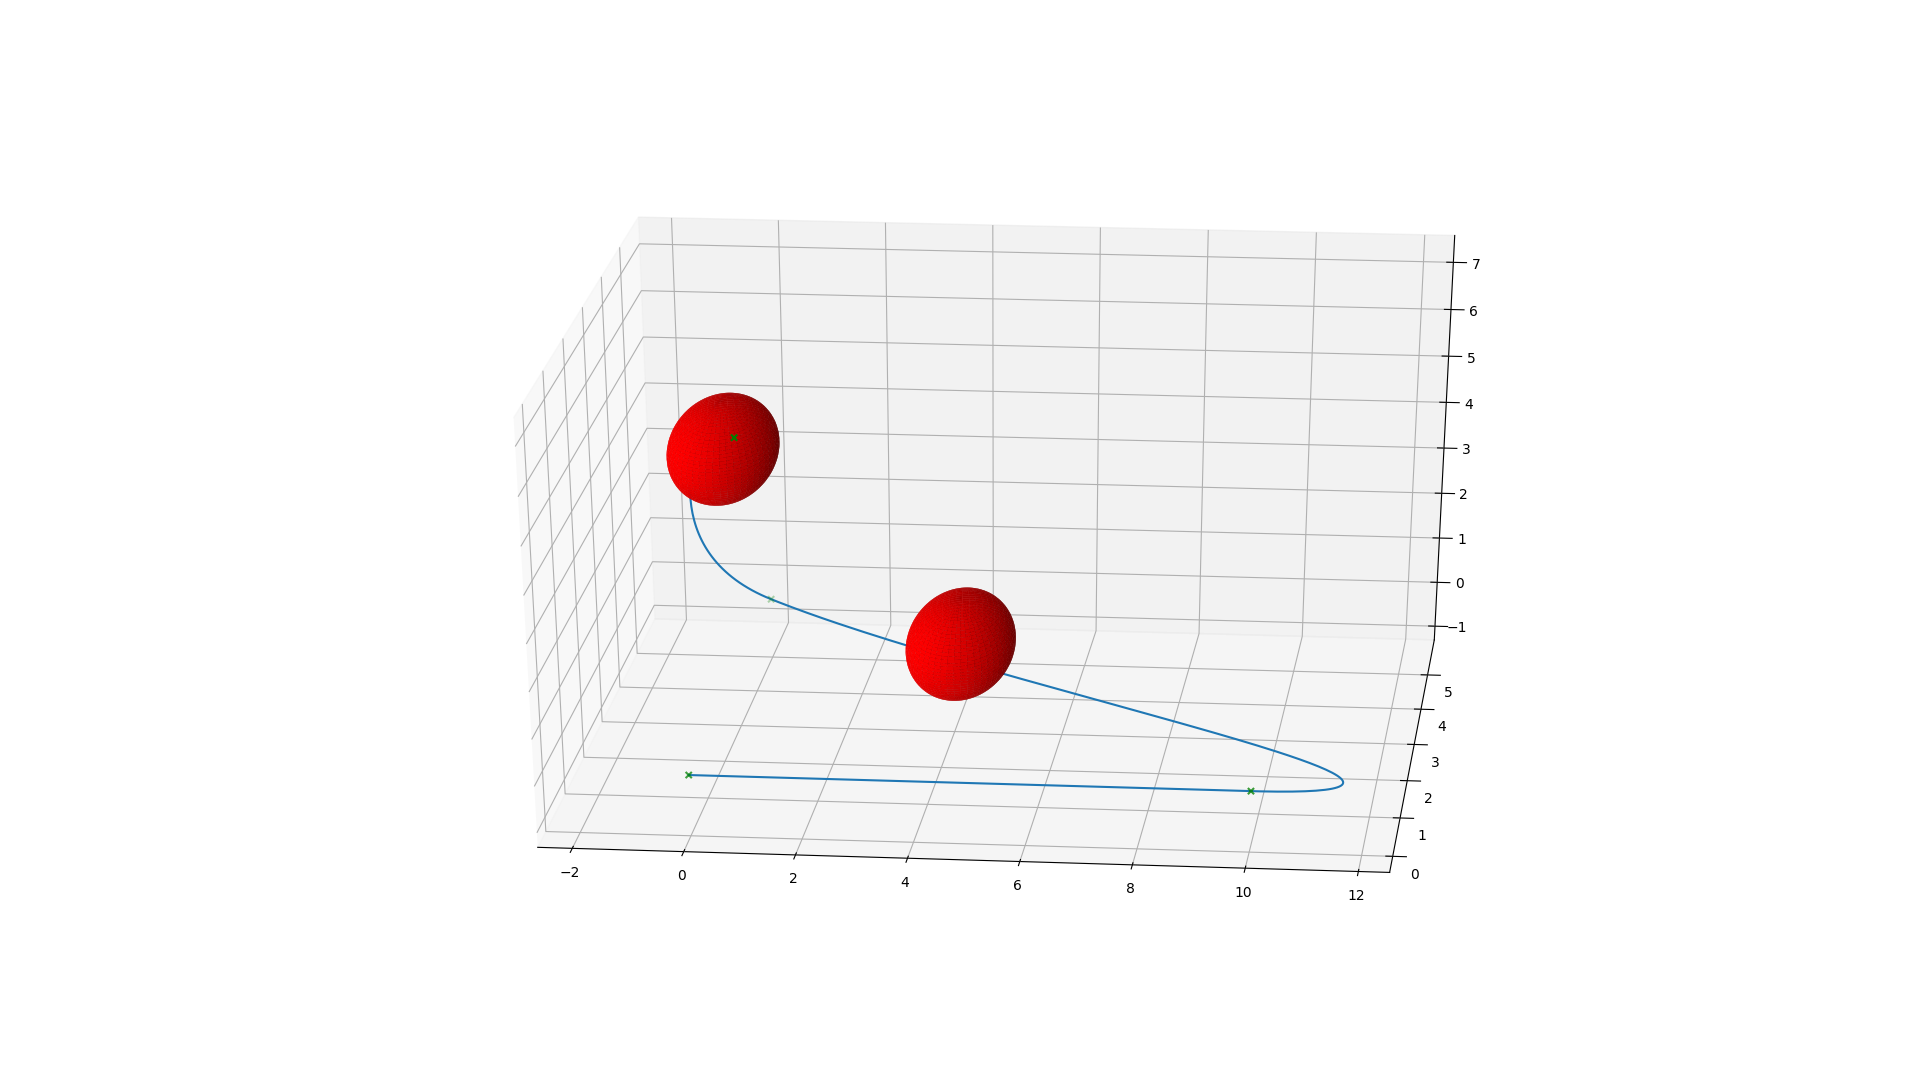
\includegraphics[width=\linewidth]{diff_flat.png}  
          \caption{Original trajectory but shows the intersecting obstacle}
          \label{fig:diff_flat}
    \end{subfigure}
    \begin{subfigure}{0.5\textwidth}
          \centering
          % include first image
          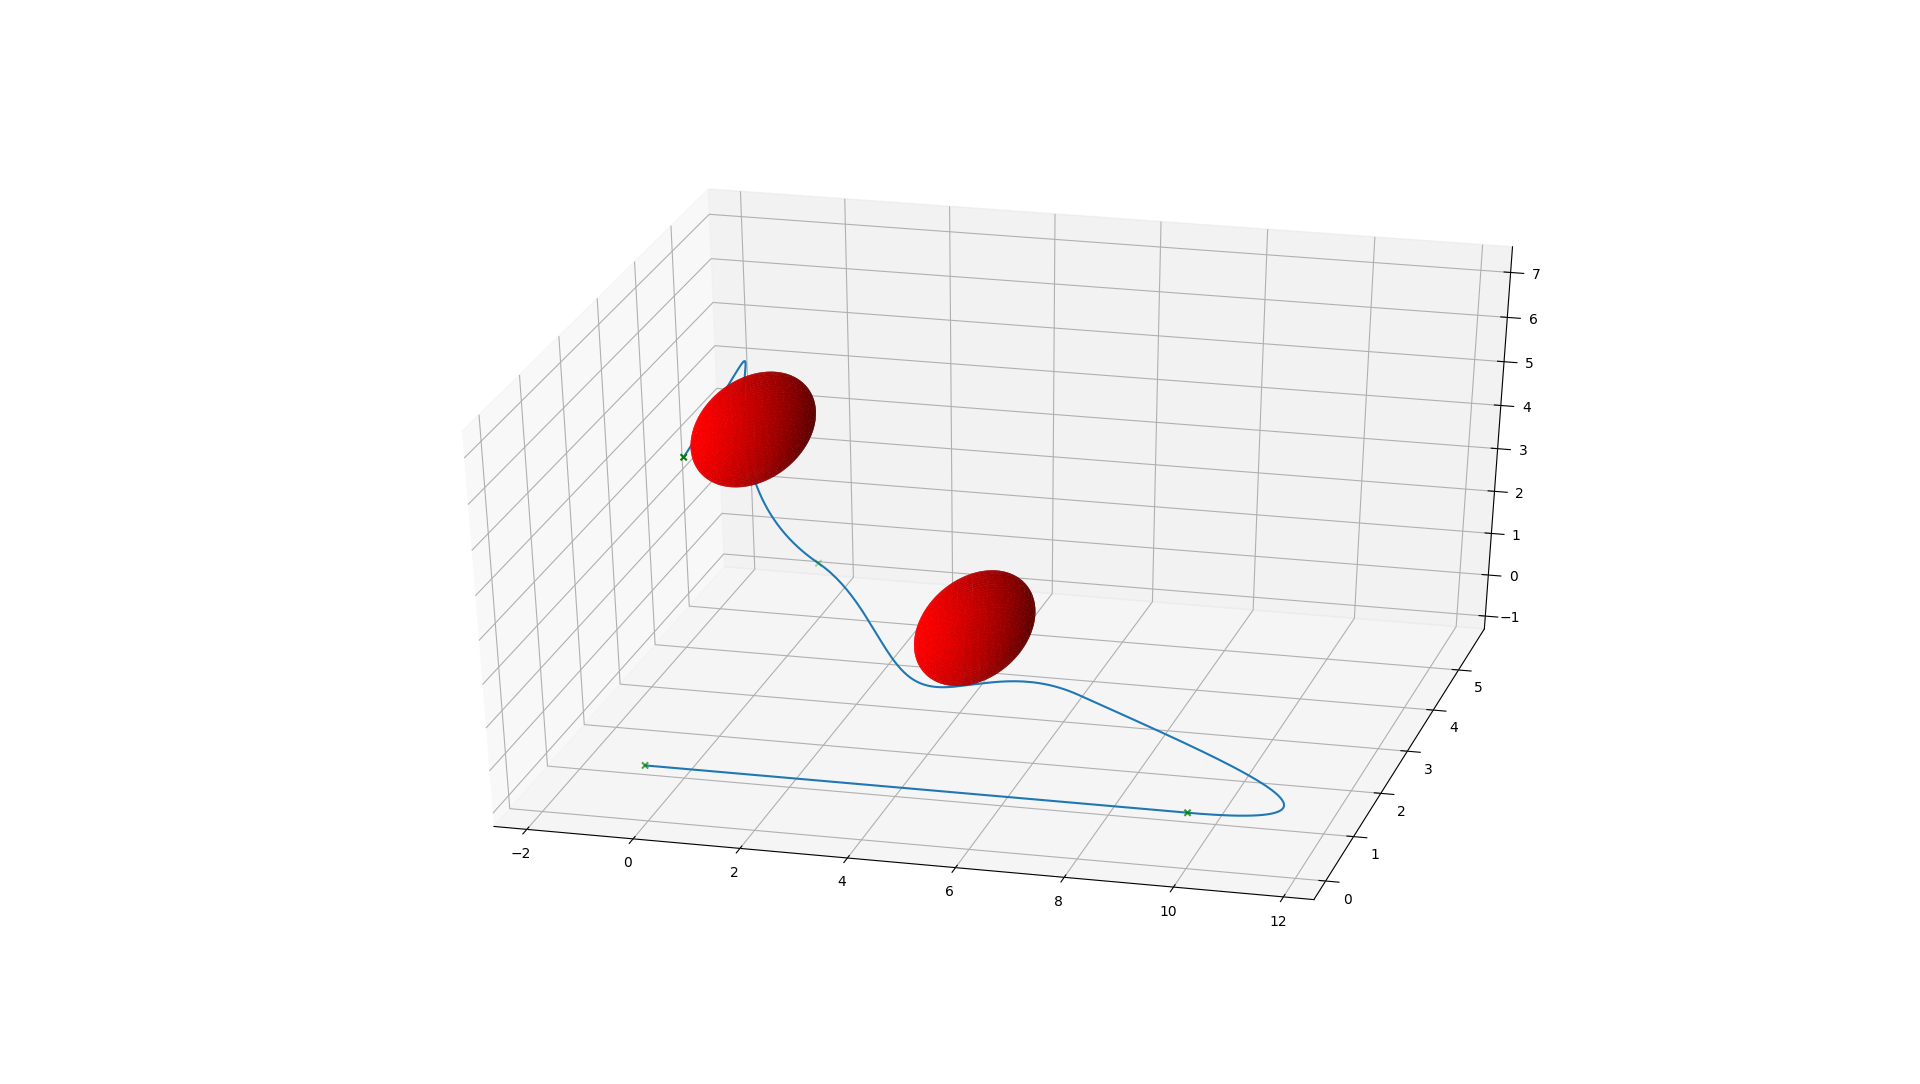
\includegraphics[width=\linewidth]{diff_flat_obst.png}  
          \caption{New optimal trajectory avoiding the obstacle}
          \label{fig:diff_flat_obst}
    \end{subfigure}
    \caption{Comparison of the trajectory before and after obstacle avoidance is applied}
    \label{fig:obst_avoid}
\end{figure}

\Cref{tab:obst_times} contains a table comparing the run times for CVXPY and SNOPT. As can be seen, CVXPY runs much faster but does not have any constraints about avoiding obstacles. SNOPT ran many times slower but does take obstacles into consideration. This is the reasoning for our two step approach. CVXPY runs the optimization quickly and checks to see if the resulting trajectory collides with a known obstacle. If a collision would occur then the optimization is rerun using SNOPT to generate a collision free trajectory. We note that, in a faster programming language, such as C++, the convex optimizer could run in real time. However, the current formulation of the optimization is not fast enough to be run in real time. We believe that the optimization problem could be reworked into a form that can be solved real time.
% such as in \cite{richter2016polynomial}.

\begin{table}[bth]
\centering
\caption{Total run times for the different optimizations to run for all 3 trajectories}
\begin{tabular}{|c|c|c|}
\hline
                  & \textbf{\begin{tabular}[c]{@{}c@{}}CVXPY\\ (No obstacles)\end{tabular}} & \textbf{\begin{tabular}[c]{@{}c@{}}SNOPT\\ (With Obstacles)\end{tabular}} \\ \hline
\textbf{Time (s)} & 0.367                                                                   & 2.094                                                                     \\ \hline
\end{tabular}
\label{tab:obst_times}
\end{table}

The last experiment was to perform the trajectory optimization on the ordered waypoints that were output from the simulated annealing algorithm. The result can be seen in \cref{fig:final_result}. As can be seen the trajectories generated are all smooth and the obstacles are all avoided. Testing was done on multiple randomized maps and the trajectory generation was able to successfully generate trajectories in all cases. While this does not show that our framework will work for every possible case, it does show that it is robust.

\begin{figure}[bth]
    \centering
    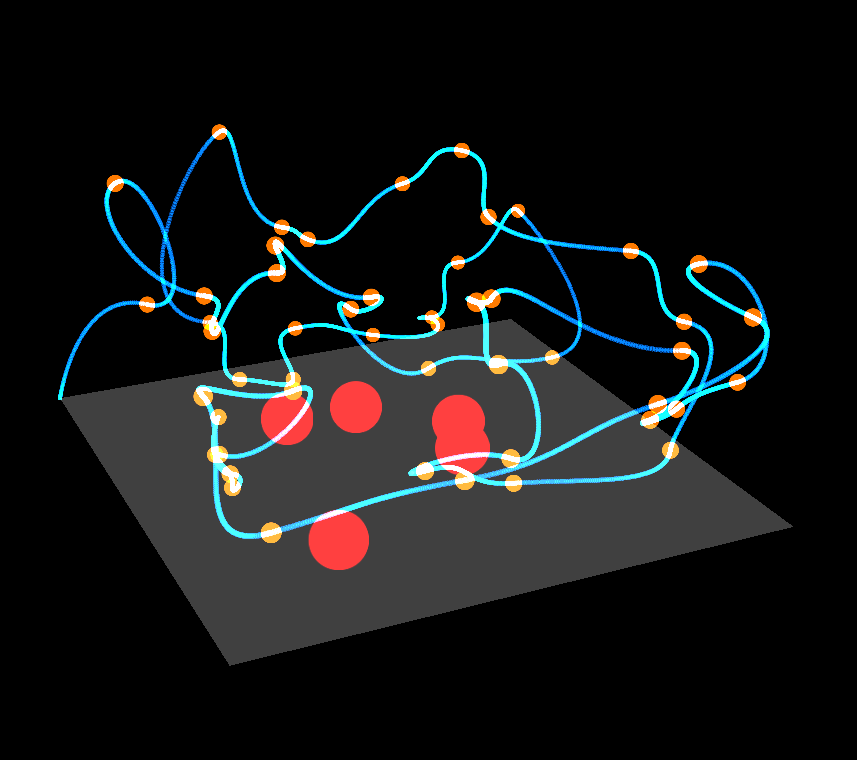
\includegraphics[width=0.9\linewidth]{project_final.png}
    \caption{50 sequential trajectories generated by the trajectory generator}
    \label{fig:final_result}
\end{figure}

\section{Conclusion}

We have presented a framework which will determine the order in which a given set of waypoints should be visited to minimize the total distance traveled and then generate dynamically feasible trajectories between them. The simulated annealing solution to the traveling salesman problem worked well by decreasing the total distance traveled to about one third of the original distance for a low computational cost. The trajectory generation also performed well in producing dynamically feasible trajectories while avoiding obstacles. One improvement to our work would be to reformulate the non-linear obstacle avoidance constraints in such a way that they become linear or incorporate the constraint in the cost function to yield an unconstrained problem that can be solved much faster. In addition, rather than solving for the shortest path through all waypoints, ideally, the actual energy cost would be the objective in the simulated annealing algorithm. This approach would take into account the different energy costs of increasing, decreasing, or maintaining altitude when travelling from one waypoint to another in 3D space.

% \IEEEtriggeratref{16}
\bibliographystyle{IEEEtran}
\bibliography{IEEEabrv,library}

\end{document}
